\documentclass[aspectratio=169,10pt]{beamer}
\usepackage[T1]{fontenc}
\usepackage[utf8]{inputenc}
\usepackage{lmodern}
\usepackage{amsmath,amssymb}
\usepackage{graphicx}
\usepackage{booktabs}
\usepackage{listings}
\usepackage{xcolor}
\usepackage{tikz}
\usetikzlibrary{arrows.meta,positioning,shapes.geometric,calc}
\usetheme{metropolis}
\metroset{progressbar=frametitle,sectionpage=none,numbering=fraction}

\title{Optimization Methods for Thermal Sciences}
\subtitle{A panorama of principles, algorithms and code}
\author{Whady Felipe Florez}
\institute{[Seminar / institution]}
\date{}

\lstdefinestyle{py}{
  language=Python,
  basicstyle=\ttfamily\fontsize{6.6}{7.7}\selectfont,
  keywordstyle=\color{blue!70!black}\bfseries,
  commentstyle=\color{gray},
  stringstyle=\color{orange!70!black},
  showstringspaces=false, breaklines=false, frame=single, framerule=0.3pt,
  tabsize=2, xleftmargin=0pt, xrightmargin=0pt, aboveskip=2pt, belowskip=2pt,
  morekeywords={as}
}
\lstset{style=py}
\newcommand{\codesz}[3]{\lstinputlisting[style=py,basicstyle=\ttfamily\fontsize{#1}{#2}\selectfont]{snippets/#3.py}}
\newcommand{\code}[1]{\codesz{6.6}{7.7}{#1}}
\newcommand{\grad}{\nabla}
\newcommand{\R}{\mathbb{R}}
\newcommand{\norm}[1]{\left\lVert #1\right\rVert}
\newcommand{\xs}{x^{\ast}}
\newcommand{\fig}[2][\linewidth]{\includegraphics[width=#1]{figs/#2}}
\setbeamertemplate{caption}{\insertcaption}

\begin{document}
\maketitle

\begin{frame}{Outline}
  \tableofcontents
\end{frame}

% =============================================================== 1
\section{Setting the stage}

\begin{frame}{Why optimization in the thermal sciences?}
  Every thermal design is a \textbf{compromise}: more insulation, more heat-exchanger area or more collector area costs money; too little wastes energy.
  \vspace{0.2cm}
  \begin{columns}[T]
    \begin{column}{0.52\textwidth}
      \begin{itemize}
        \item How thick should the insulation on a steam line be?
        \item How large a heat-recovery exchanger, and at what water flow?
        \item At what temperature should a solar field operate?
        \item Where should a temperature-sensitive part go on a hot board?
        \item Which $h$, $k$, $\varepsilon$ best fit my measured cooling curve?
      \end{itemize}
    \end{column}
    \begin{column}{0.44\textwidth}
      \begin{alertblock}{Today's goal}
        A \textbf{map} of the main families of methods, one clear \emph{picture} and one short \emph{code} per method, all on thermal problems.
      \end{alertblock}
      \small No heavy theory: what each method \textbf{does}, \textbf{when} it works and \textbf{when} it fails.
    \end{column}
  \end{columns}
\end{frame}

\begin{frame}{Anatomy of an optimization problem}
  \[ \min_{x\in\R^n}\ f(x)\qquad\text{subject to}\qquad g_j(x)\le 0,\quad h_i(x)=0 \]
  \begin{itemize}
    \item $x$: the \textbf{decision variables}, a \emph{vector} (thickness, area and flow, a position, \dots)
    \item $f(x)$: the \textbf{objective}: a single number to minimise (annual cost, temperature, exergy loss)
    \item $g(x)\le0,\ h(x)=0$: the \textbf{constraints} (maximum temperature, demand to be met, energy balance)
  \end{itemize}
  \begin{center}\small
  \begin{tabular}{llll}
    \toprule
    Problem & $x$ & $f(x)$ & constraint\\
    \midrule
    P1 insulation & $[t]$ & energy lost + insulation cost & --\\
    P2 component placement & $[x_1,x_2]$ & board temperature & inside the board\\
    P3 heat recovery & $[a,\,m]$ & area + pumping $-$ heat value & --\\
    P4 solar field & $[A,\ \Delta T]$ & area cost $-$ premium for hot heat & demand $\le A\,G\,\eta(\Delta T)$\\
    \bottomrule
  \end{tabular}
  \end{center}
\end{frame}

\begin{frame}{Four thermal test problems used throughout}
  \begin{columns}[T]
    \begin{column}{0.60\textwidth}
      \fig{fig_problems_overview.png}
    \end{column}
    \begin{column}{0.38\textwidth}
      \small
      \textbf{P1} \emph{1-D, unimodal}: golden section.\\[3pt]
      \textbf{P2} \emph{2-D, several valleys}: Metropolis, simulated annealing, Great Deluge.\\[3pt]
      \textbf{P3} \emph{2-D, smooth narrow valley}: gradient descent, Newton, dogleg, simplex.\\[3pt]
      \textbf{P4} \emph{2-D, constrained}: cutting plane, penalty and barrier.\\[6pt]
      \footnotesize Physical models are deliberately simple (closed-form), so the \emph{method} is the star, not the model.
    \end{column}
  \end{columns}
\end{frame}

\begin{frame}{P1: how thick should the insulation be?}
  \begin{columns}[T]
    \begin{column}{0.5\textwidth}
      \small
      Bare steam pipe ($r_1=5$ cm, 180\,$^\circ$C) in 20\,$^\circ$C air. Insulation of thickness $t$ ($k=0.045$ W/m\,K):
      \[ q'(t)=\frac{T_f-T_\infty}{\dfrac{\ln(r_2/r_1)}{2\pi k}+\dfrac{1}{2\pi r_2 h}},\quad r_2=r_1+t \]
      \[ f(t)=\underbrace{c_E\,q'(t)\,H}_{\text{energy lost}}+\underbrace{\mathrm{CRF}\,c_V\,\pi(r_2^2-r_1^2)}_{\text{insulation}} \]
      \footnotesize $H=8000$ h/yr, $c_E=0.04$ \$/kWh, $c_V=2500$ \$/m$^3$, CRF $=0.2$.
      \normalsize
      \begin{itemize}
        \item More insulation: less energy lost, more capital.
        \item Bare pipe: 161 \$/m/yr. Optimum: 31 \$/m/yr.
      \end{itemize}
    \end{column}
    \begin{column}{0.48\textwidth}
      \fig{fig_P1_cost.png}
    \end{column}
  \end{columns}
\end{frame}

\begin{frame}{P2: where to mount a temperature-sensitive component?}
  \begin{columns}[T]
    \begin{column}{0.46\textwidth}
      \small
      Thin board ($k=20$ W/m\,K, 2 mm) with 5 hot chips and 4 cooled clamps. Fin-type conduction gives, for each source $q_j$ (W):
      \[ T(x)=T_0+\sum_j\frac{q_j}{2\pi k\,t_b}\,K_0\!\bigl(m\,\|x-x_j\|\bigr) \]
      with $m=\sqrt{2h/(k\,t_b)}$ and $q_j<0$ for clamps.
      \begin{itemize}
        \item Goal: \textbf{minimise} $T(x)$, $x=[x_1,x_2]$ in the board.
        \item \textbf{Four local minima} (circled), one global: $(12.0,\,2.7)$\,cm, $24.4\,^\circ$C.
        \item The other three: 43--46\,$^\circ$C.
      \end{itemize}
    \end{column}
    \begin{column}{0.52\textwidth}
      \fig{fig_P2_landscape.png}
    \end{column}
  \end{columns}
\end{frame}

\begin{frame}{P3: heat-recovery exchanger (area and water flow)}
  \begin{columns}[T]
    \begin{column}{0.5\textwidth}
      \small
      Hot exhaust (20 kW/K, 250\,$^\circ$C) heats water of flow $m$ in a counter-flow exchanger of area $A=50\,a$ m$^2$ ($\varepsilon$--NTU):
      \[ \mathrm{NTU}=\frac{UA}{m c_p},\quad U=U_0\,m^{0.8},\quad Q=\varepsilon\,m c_p\,(T_h-T_c) \]
      \[ f(a,m)=\underbrace{c_A A}_{\text{area}}+\underbrace{c_p\,m^{2.8}}_{\text{pumping}}-\underbrace{c_Q\,Q}_{\text{value of heat}} \]
      \begin{itemize}
        \item Optimum: $A=220$ m$^2$, $m=1.44$ kg/s, $Q=1.35$ MW, net gain $93.6$ k\$/yr.
        \item A narrow curved valley: area and flow compensate each other.
        \item Hessian condition number $\approx 65$ at the optimum.
      \end{itemize}
    \end{column}
    \begin{column}{0.48\textwidth}
      \fig{fig_P3_landscape.png}
    \end{column}
  \end{columns}
\end{frame}

\begin{frame}{P4: solar collector field, constrained}
  \begin{columns}[T]
    \begin{column}{0.5\textwidth}
      \small
      Process heat of $Q_{dem}=100$ kW from collectors ($G=800$ W/m$^2$) with efficiency $\eta(\Delta T)=\eta_0-a_1\tfrac{\Delta T}{G}-a_2\tfrac{\Delta T^2}{G}$.
      \[ \min\ 5\,x_1-2\,x_2\quad\text{s.t.}\quad \underbrace{\frac{Q_{dem}}{G\,\eta(10x_2)}\cdot\frac1{100}-x_1}_{g(x)}\le0 \]
      $x_1=A/100$ m$^2$ (area cost 5 k\$/yr per unit), $x_2=\Delta T/10$ K (credit of 2 k\$/yr per unit: hotter heat is worth more).
      \begin{itemize}
        \item Optimum on the boundary: $A=275$ m$^2$, $\Delta T=59.4$ K, $\eta=0.454$.
        \item $g$ is \textbf{convex}: the feasible set is convex.
      \end{itemize}
    \end{column}
    \begin{column}{0.48\textwidth}
      \fig{fig_P4_feasible.png}
    \end{column}
  \end{columns}
\end{frame}

\begin{frame}[fragile]{The convention for all the code: $f(x)$ with $x$ a vector}
  \small Every method below receives \textbf{only a function of one vector}, a black box:
\begin{lstlisting}
def cost_insulation(x):                       # P1: x = [t]
    r2 = R1 + x[0]
    R_th = np.log(r2 / R1) / (2*np.pi*K_INS) + 1.0 / (2*np.pi*r2*H_OUT)
    energy  = (T_FLUID - T_AMB) / R_th / 1000.0 * HOURS * C_ENERGY
    capital = C_VOL * np.pi * (r2**2 - R1**2) * CRF
    return energy + capital

def temperature_board(x):                     # P2: x = [x1, x2]  (cm)
    d = np.sqrt(np.sum((x - SRC[:, :2])**2, axis=1) + R0**2)       # distance to every source
    return T_BASE + np.sum(SRC[:, 2] / (2*np.pi*K_PLATE*THK) * k0(M_FIN * d))

def cost_exchanger(x):                        # P3: x = [a, m]
    A, m = 50.0 * x[0], x[1]
    return (C_AREA*A + C_PUMP*m**2.8 - C_HEAT*exchanger_duty(x)/1000.0) / 1000.0
\end{lstlisting}
  Same signature for 1, 2 or 200 variables: \texttt{f(x)}. Methods never see the physics; they only call $f$.
\end{frame}

\begin{frame}{A map of the methods}
  \centering
  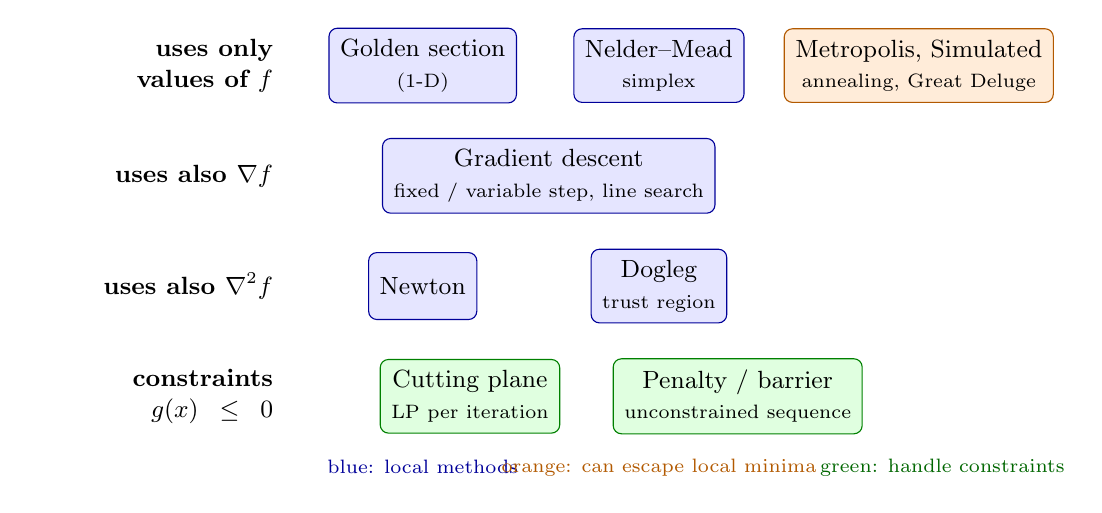
\begin{tikzpicture}[
      lab/.style={font=\small\bfseries, text width=3.0cm, align=right},
      box/.style={draw, rounded corners=3pt, align=center, minimum height=0.85cm, font=\small, inner sep=4pt},
      glob/.style={box, fill=orange!15, draw=orange!70!black},
      loc/.style={box, fill=blue!10, draw=blue!60!black},
      con/.style={box, fill=green!12, draw=green!50!black}]
    \node[lab] at (0,3.6) {uses only values of $f$};
    \node[loc] at (3.4,3.6) {Golden section\\ \scriptsize(1-D)};
    \node[loc] at (6.4,3.6) {Nelder--Mead\\ \scriptsize simplex};
    \node[glob] at (9.7,3.6) {Metropolis, Simulated\\ \scriptsize annealing, Great Deluge};
    \node[lab] at (0,2.2) {uses also $\grad f$};
    \node[loc] at (5.0,2.2) {Gradient descent\\ \scriptsize fixed / variable step, line search};
    \node[lab] at (0,0.8) {uses also $\grad^2 f$};
    \node[loc] at (3.4,0.8) {Newton};
    \node[loc] at (6.4,0.8) {Dogleg\\ \scriptsize trust region};
    \node[lab] at (0,-0.6) {constraints $g(x)\le 0$};
    \node[con] at (4.0,-0.6) {Cutting plane\\ \scriptsize LP per iteration};
    \node[con] at (7.4,-0.6) {Penalty / barrier\\ \scriptsize unconstrained sequence};
    \node[font=\scriptsize, text=blue!60!black] at (3.4,-1.5) {blue: local methods};
    \node[font=\scriptsize, text=orange!70!black] at (6.4,-1.5) {orange: can escape local minima};
    \node[font=\scriptsize, text=green!40!black] at (10.0,-1.5) {green: handle constraints};
  \end{tikzpicture}
\end{frame}

\begin{frame}{Local versus global: why the landscape matters}
  \begin{columns}[T]
    \begin{column}{0.5\textwidth}
      \begin{itemize}
        \item A \textbf{local} method stops in the valley where it starts. Start near $(23,8)$\,cm: it ends at \textbf{43\,$^\circ$C}, although $24$\,$^\circ$C exists elsewhere.
        \item Smooth \emph{unimodal} problems (P1, P3): local methods are enough, and the fastest ones win.
        \item \emph{Multimodal} problems (P2): we need a method that sometimes accepts a \textbf{worse} point.
      \end{itemize}
      \begin{alertblock}{Rule of thumb}
        First plot (or sample) $f$. If you see several valleys, think \textbf{global}; if one smooth valley, think \textbf{Newton-like}.
      \end{alertblock}
    \end{column}
    \begin{column}{0.48\textwidth}
      \fig{fig_P2_landscape.png}
    \end{column}
  \end{columns}
\end{frame}

% =============================================================== 2
\section{Golden-section search}

\begin{frame}{Golden section: the simplest method (1-D, no derivatives)}
  \begin{itemize}
    \item Assume $f$ is \textbf{unimodal} on $[a,b]$ (one valley). Evaluate two interior probes $x_1<x_2$.
    \item If $f(x_1)<f(x_2)$ the minimum is in $[a,x_2]$; otherwise in $[x_1,b]$. \textbf{Discard the rest.}
    \item Choose the probes at $x_1=b-r(b-a)$, $x_2=a+r(b-a)$ with $r=\frac{\sqrt5-1}{2}=0.618\dots$
  \end{itemize}
  \begin{alertblock}{Why the golden ratio?}
    With this $r$ one surviving probe lands \textbf{exactly} on a probe of the next iteration: only \textbf{one new evaluation} per iteration, and the bracket shrinks by $0.618$ each time.
  \end{alertblock}
  \small Thermal use: any one-parameter design with a single optimum (insulation thickness, fin length, optimal flow rate).
\end{frame}

\begin{frame}{Golden section on P1: iteration by iteration}
  \centering
  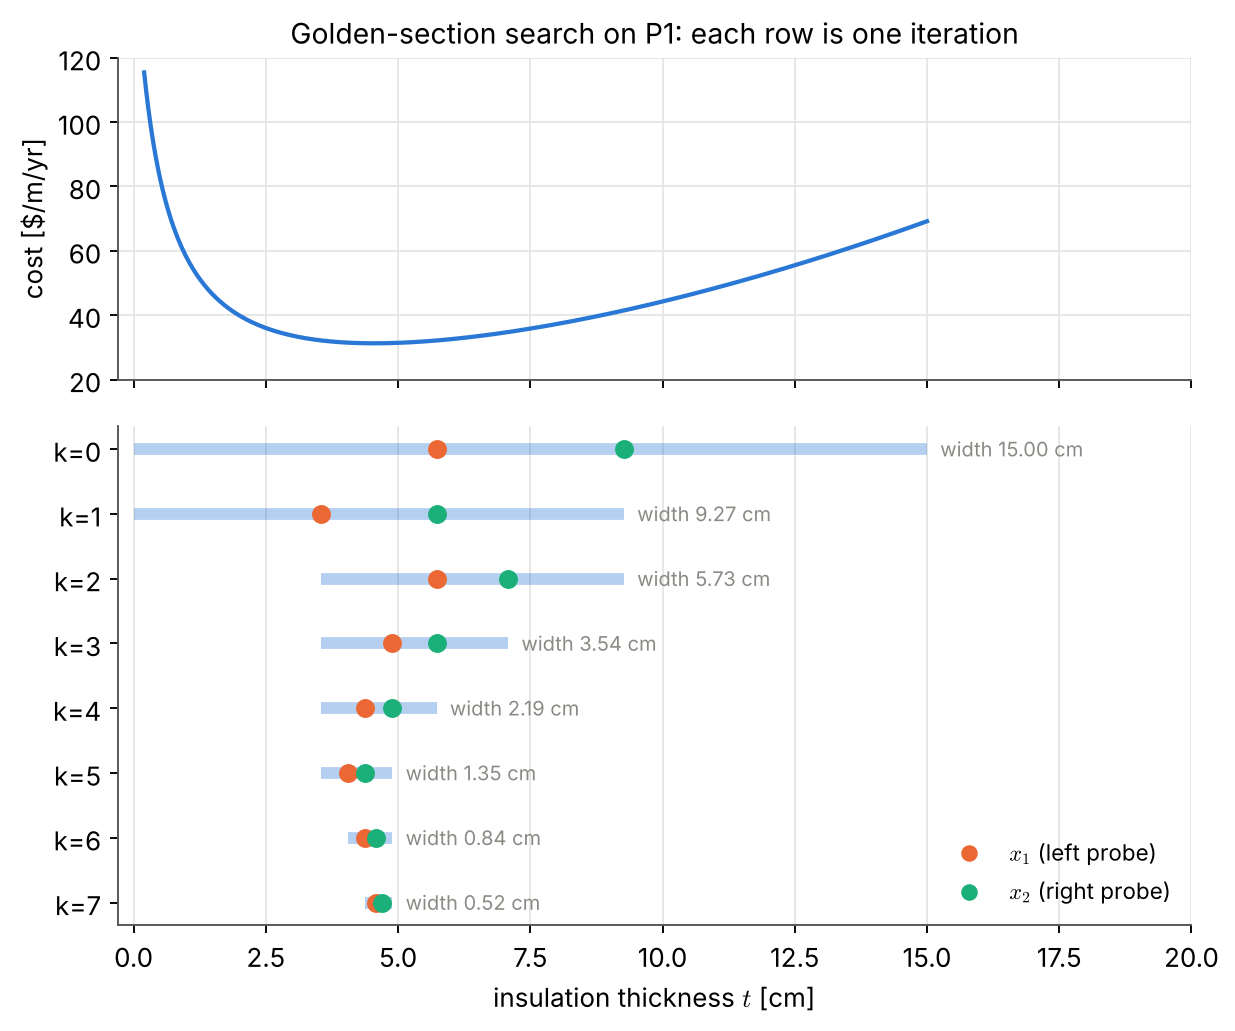
\includegraphics[height=6.5cm]{figs/fig_golden_iter.png}
\end{frame}

\begin{frame}{Golden section: the code}
  \code{golden}
  \small \texttt{f} takes a vector (\texttt{f(np.array([t]))}); \texttt{f1}, \texttt{f2} are \textbf{reused}, never recomputed.
\end{frame}

\begin{frame}{Golden section: result and cost}
  \begin{columns}[T]
    \begin{column}{0.48\textwidth}
      \small
      \begin{center}
      \begin{tabular}{lrr}
        \toprule
        & manual & \texttt{scipy} golden\\
        \midrule
        $t^\ast$ [cm] & 4.549 & 4.548\\
        $f(t^\ast)$ [\$/m/yr] & 31.2518 & 31.2518\\
        iterations & 16 & 20\\
        $f$ evaluations & 18 & 25\\
        \bottomrule
      \end{tabular}
      \end{center}
      Bracket $[0,15]$ cm $\to$ $0.1$ mm.
      \begin{itemize}
        \item Robust, no derivatives; linear convergence ($0.618$ per evaluation).
        \item Fails silently if $f$ has several valleys in the bracket.
      \end{itemize}
      \footnotesize \texttt{minimize\_scalar(method="golden")}
    \end{column}
    \begin{column}{0.5\textwidth}
      \fig{fig_golden_conv.png}
    \end{column}
  \end{columns}
\end{frame}

% =============================================================== 3
\section{Escaping local minima: Metropolis, annealing, Deluge}

\begin{frame}{The problem: a valley is not the best valley}
  \begin{columns}[T]
    \begin{column}{0.5\textwidth}
      \begin{itemize}
        \item P2: start at $x_0=(23,\,8)$ cm, in a shallow cold pocket near a clamp ($43.4\,^\circ$C).
        \item Any method that only accepts \textbf{improvements} (``greedy'') stays there: every neighbour is hotter.
        \item To reach the cold region near $(12,\,2.7)$ we must first \textbf{climb} through $\approx$55\,$^\circ$C.
      \end{itemize}
      \begin{alertblock}{Key idea}
        Accept an \textbf{uphill} move sometimes, with a probability that depends on how bad it is.
      \end{alertblock}
    \end{column}
    \begin{column}{0.5\textwidth}
      \fig{fig_P2_landscape.png}
    \end{column}
  \end{columns}
\end{frame}

\begin{frame}{The thermodynamic idea (Metropolis, 1953)}
  \begin{columns}[T]
    \begin{column}{0.55\textwidth}
      \begin{itemize}
        \item A system at temperature $T$ visits a state of energy $E$ with probability
        \[ p(E)\propto e^{-E/(k_BT)} \qquad\text{(Boltzmann)} \]
        \item \textbf{Metropolis} built a simple random walk whose visits follow exactly this law:
        \begin{itemize}
          \item propose a random move $x\to x'$, $\Delta E=f(x')-f(x)$;
          \item \textbf{accept} it if $\Delta E\le0$;
          \item otherwise accept with probability $e^{-\Delta E/T}$.
        \end{itemize}
        \item Here $f$ plays the role of energy and $T$ is a ``temperature'' in the units of $f$ ($^\circ$C for P2).
      \end{itemize}
    \end{column}
    \begin{column}{0.43\textwidth}
      \fig{fig_metropolis_prob.png}
    \end{column}
  \end{columns}
\end{frame}

\begin{frame}{Metropolis: the code}
  \code{metropolis}
\end{frame}

\begin{frame}{A chain at fixed $T$ samples the Boltzmann distribution}
  \centering
  \fig[0.80\linewidth]{fig_boltzmann_P1.png}\\[2pt]
  \small Check on P1: histogram of 150\,000 Metropolis steps (blue) against the theoretical $e^{-f/T}$ (orange).\\
  Low $T$: the chain hugs the minimum. High $T$: it wanders widely. \textbf{$T$ is the exploration knob.}
\end{frame}

\begin{frame}{Fixed temperature on P2: exploration versus exploitation}
  \centering
  \fig[0.97\linewidth]{fig_metropolis_P2.png}
  \begin{itemize}
    \item $T\approx0$ (greedy): stuck at 43.4\,$^\circ$C. $\;T=3$: crosses to the cold region and stays. $\;T=20$: accepts almost everything and never settles.
    \item Too cold = trapped; too hot = random walk. The right $T$ depends on the \textbf{barrier heights} of the problem.
  \end{itemize}
\end{frame}

\begin{frame}{Simulated annealing: cool the temperature as you go}
  \small
  A Metropolis chain with a \textbf{decreasing} temperature, as when a metal is cooled slowly into a low-energy lattice:
  $T_k=T_0\,\alpha^{k}$, $0<\alpha<1$. Hot $\to$ explores; cold $\to$ refines. Keep the \textbf{best point ever seen}.\\[8pt]
  \codesz{7.3}{8.6}{sa}
  \footnotesize Parameters: $T_0\approx$ barrier height, $\alpha$ such that $T_{end}$ is small, step $\approx$ feature size.
\end{frame}

\begin{frame}{Simulated annealing on P2}
  \begin{columns}[T]
    \begin{column}{0.5\textwidth}\fig{fig_sa_path.png}\end{column}
    \begin{column}{0.48\textwidth}\fig{fig_sa_schedule.png}\end{column}
  \end{columns}
  \small $T_0=20\,^\circ$C, $\alpha=0.997$, 2000 steps, step size 1 cm. Start $(23,8)$ $\to$ best $24.4\,^\circ$C at $(12.0,\,2.7)$.
\end{frame}

\begin{frame}{Great Deluge (Dueck, 1993): a flood instead of a temperature}
  \begin{columns}[T]
    \begin{column}{0.33\textwidth}
      \footnotesize
      \begin{itemize}
        \item Picture a hiker in a landscape while a flood level \textbf{sinks} steadily.
        \item Accept \textbf{any} move whose $f$ is below the level: no probabilities, no $T$.
        \item The level falls by a fixed ``rain'' each step, from a high start to a \textbf{target} value.
        \item The region shrinks into separate ponds; the walker ends in the one it is in.
      \end{itemize}
      \begin{alertblock}{Parameters}
        start level, \textbf{target}, step: the target is an \emph{engineering goal} (here 26\,$^\circ$C).
      \end{alertblock}
    \end{column}
    \begin{column}{0.65\textwidth}
      \fig{fig_deluge.png}
    \end{column}
  \end{columns}
\end{frame}

\begin{frame}{Great Deluge: the code}
  \codesz{7.3}{8.8}{deluge}\vspace{4pt}
  \small Note how short it is: one comparison \texttt{f\_new <= level} replaces the whole Metropolis probability.
\end{frame}

\begin{frame}{Head to head on P2 (same start, same budget)}
  \begin{columns}[T]
    \begin{column}{0.62\textwidth}
      \fig{fig_stochastic_compare.png}
    \end{column}
    \begin{column}{0.36\textwidth}
      \small
      \begin{itemize}
        \item 60 seeds, 2000 evaluations each, start $(23,8)$, step 1 cm; success: $f<26\,^\circ$C.
        \item Greedy: \textbf{never} escapes.
        \item If we \textbf{remember the best point}, any $T$ high enough to cross the barriers finds the cold region (95--100\%).
        \item But \textbf{where the walker ends} is another story: only SA \emph{ends} cold (75\%).
        \item Great Deluge: 63\% / 42\%.
      \end{itemize}
      \footnotesize Judge stochastic methods over many seeds, never one run.
    \end{column}
  \end{columns}
\end{frame}

\begin{frame}{What does the temperature knob really do?}
  \centering
  \fig[0.80\linewidth]{fig_T_sweep.png}
  \small
  \begin{itemize}
    \item \textbf{Best visited:} fixed $T\ge3$ already finds the cold region; SA needs a hot enough start ($T_0\gtrsim10$), because it cools while exploring. Too cold ($T\le1$): trapped.
    \item \textbf{Final position:} a fixed-$T$ chain ends wherever thermal noise puts it (best $\approx40\%$ at $T=2$--3, nearly 0 when hotter). SA's final state is good ($\approx80\%$) \emph{without} bookkeeping, because it cools into the minimum.
  \end{itemize}
\end{frame}

\begin{frame}[fragile]{In \texttt{scipy} and in practice}
\begin{lstlisting}
from scipy.optimize import dual_annealing
res = dual_annealing(temperature_board, bounds=[(0, 24), (0, 16)], seed=0, maxfun=2000)
print(res.x, res.fun)          # -> [12.04  2.70]   24.38 C
\end{lstlisting}
  \begin{itemize}
    \item \texttt{dual\_annealing} (generalised SA plus a local polish) reaches the same optimum as our manual code.
    \item Practical advice: choose \textbf{step} from the feature size of $f$, $T_0$ from a typical \textbf{barrier}, $T_{end}$ from the resolution you need; run \textbf{many seeds}; keep the best point; finish with a local method.
    \item Cost: thousands of evaluations; use them when $f$ is cheap, derivatives unavailable, or valleys abound.
  \end{itemize}
\end{frame}

% =============================================================== 4
\section{Gradient-based methods: descent, Newton, dogleg}

\begin{frame}{Using derivatives: back to the smooth valley (P3)}
  \begin{columns}[T]
    \begin{column}{0.5\textwidth}
      \begin{itemize}
        \item $\grad f(x)$ points \textbf{uphill}; $-\grad f$ is the direction of fastest local decrease.
        \item General descent iteration:
        \[ x_{k+1}=x_k+\alpha_k\,p_k,\qquad p_k=-\grad f(x_k) \]
        \item The art is in the \textbf{step length} $\alpha_k$ (and, later, in a better direction $p_k$).
        \item Derivatives are not magic: from a black-box $f(x)$ we get them by \textbf{finite differences}.
      \end{itemize}
    \end{column}
    \begin{column}{0.48\textwidth}
      \fig{fig_P3_landscape.png}
    \end{column}
  \end{columns}
\end{frame}

\begin{frame}{Derivatives of a black box: finite differences}
  \codesz{7.6}{9}{numgrad}
  \small Central difference $\frac{f(x+he_i)-f(x-he_i)}{2h}$: $2n$ evaluations. The Hessian differences the gradient.
\end{frame}

\begin{frame}{Fixed step: the step length decides everything}
  \begin{columns}[T]
    \begin{column}{0.56\textwidth}
      \fig{fig_gd_paths.png}
    \end{column}
    \begin{column}{0.42\textwidth}
      \small
      \begin{itemize}
        \item $\alpha=0.01$: converges, but \textbf{500 iterations} are not enough (error still $10^{-5}$).
        \item $\alpha=0.02$: \textbf{diverges} in 8 iterations (leaves the valid region).
        \item Stability limit: $\alpha<2/\lambda_{\max}(H)$. Here $\lambda_{\max}\approx145$, so $\alpha<0.0138$.
        \item Narrow valley (condition number $\approx65$): steepest descent \textbf{zig-zags}.
      \end{itemize}
      \begin{alertblock}{Lesson}
        A step that is good now may be terrible later. Use a \textbf{variable} step.
      \end{alertblock}
    \end{column}
  \end{columns}
\end{frame}

\begin{frame}{Variable step: prescribed decay or line search}
  \begin{columns}[T]
    \begin{column}{0.5\textwidth}
      \begin{block}{Prescribed decay}
        $\alpha_k=\dfrac{\alpha_0}{1+0.05\,k}$: cheap, but you must guess $\alpha_0$ and the rate (stalls in the example: error $0.06$ after 500 its.).
      \end{block}
      \begin{block}{Line search (backtracking Armijo)}
        Start with a large $\alpha$ and \textbf{halve it} until the decrease is \emph{sufficient}:
        \[ f(x+\alpha p)\le f(x)+c_1\,\alpha\,\grad f^\top p,\quad c_1=10^{-4} \]
        Adapts to the local scale automatically; costs a few extra evaluations per iteration.
      \end{block}
    \end{column}
    \begin{column}{0.48\textwidth}
      \fig{fig_linesearch.png}\\[-2pt]
      \scriptsize Trial steps $\alpha=1,\,\tfrac12,\,\tfrac14,\,\tfrac18,\,\tfrac1{16}$ are rejected; $\alpha=\tfrac1{32}$ is accepted.
    \end{column}
  \end{columns}
\end{frame}

\begin{frame}{Backtracking line search: the code}
  \codesz{9}{11}{linesearch}\vspace{6pt}
  \small Five lines: the whole of the Armijo rule. \texttt{g @ p} is the slope $\grad f^\top p$ along the step.
\end{frame}

\begin{frame}{Gradient descent with the three step rules: the code}
  \codesz{7.1}{8.4}{gd}
  \footnotesize \texttt{rule} changes only the line computing \texttt{alpha}. P3 from $(0.5,0.5)$: line search needs \textbf{242 iterations}.
\end{frame}

\begin{frame}{Newton's method: use the curvature}
  \begin{columns}[T]
    \begin{column}{0.5\textwidth}
      \begin{itemize}
        \item Replace $f$ by its \textbf{local parabola} (second-order Taylor):
        \[ m(p)=f+\grad f^\top p+\tfrac12\,p^\top H\,p \]
        \item Jump to the minimum of the parabola: solve
        \[ H\,p=-\grad f,\qquad x_{k+1}=x_k+p \]
        \item Near the optimum the error is \textbf{squared} at each step (quadratic convergence).
        \item Cost per iteration: Hessian ($n^2$ derivatives) and one linear solve.
      \end{itemize}
    \end{column}
    \begin{column}{0.48\textwidth}
      \fig{fig_newton_1d.png}\\[-2pt]
      \scriptsize P1 from $t_0=1.2$ cm: three Newton steps reach $3.93$ cm (the optimum is $4.55$).
    \end{column}
  \end{columns}
\end{frame}

\begin{frame}{Newton: the code}
  \codesz{7.0}{8.2}{newton}
  \small \texttt{safeguard=True}: shift a non-PD $H$ and backtrack. \texttt{False}: the textbook method.
\end{frame}

\begin{frame}{Newton versus gradient descent on P3}
  \begin{columns}[T]
    \begin{column}{0.58\textwidth}
      \fig{fig_conv_P3.png}
    \end{column}
    \begin{column}{0.40\textwidth}
      \small
      Same start $(0.5,0.5)$:
      \begin{center}
      \begin{tabular}{lr}
        \toprule
        method & iterations\\
        \midrule
        GD, fixed $\alpha=0.01$ & $>500$\\
        GD, line search & 242\\
        Newton (safeguarded) & 7\\
        Dogleg & 9\\
        \bottomrule
      \end{tabular}
      \end{center}
      \begin{itemize}
        \item The curve for Newton is almost \textbf{vertical}: $10^{-1}\to10^{-3}\to10^{-6}$.
        \item But each iteration needs a Hessian (here by finite differences: 206 function calls in total).
      \end{itemize}
    \end{column}
  \end{columns}
\end{frame}

\begin{frame}{When Newton fails: negative curvature}
  \begin{columns}[T]
    \begin{column}{0.58\textwidth}
      \fig{fig_newton_fail.png}
    \end{column}
    \begin{column}{0.40\textwidth}
      \small
      \begin{itemize}
        \item At small area, $f$ is \textbf{not convex}: $H$ has eigenvalues $-28$ and $+154$.
        \item The ``parabola'' opens downward in one direction: its stationary point is a \textbf{saddle}, not a minimum.
        \item Pure Newton jumps to $a<0$, $m<0$: physically meaningless (the model is invalid there).
      \end{itemize}
      \begin{alertblock}{Two cures}
        (1) Fix $H$ and line-search, (2) \textbf{limit the step} to a region where the model is trusted.
      \end{alertblock}
    \end{column}
  \end{columns}
\end{frame}

\begin{frame}{Trust region: how far do we believe the model?}
  \begin{itemize}
    \item Model $m(p)=f+g^\top p+\tfrac12p^\top Bp$ is trusted only for $\|p\|\le\Delta$ (trust-region radius).
    \item After the step, compare what the model \textbf{promised} with what actually happened:
    \[ \rho=\frac{f(x)-f(x+p)}{m(0)-m(p)}=\frac{\text{actual decrease}}{\text{predicted decrease}} \]
  \end{itemize}
  \begin{center}\small
  \begin{tabular}{lll}
    \toprule
    $\rho$ & meaning & action\\
    \midrule
    $\rho<0.25$ & model was poor & \textbf{shrink} $\Delta$ ($\times\frac14$)\\
    $\rho>0.75$ and step on the boundary & model was good & \textbf{expand} $\Delta$ ($\times2$)\\
    $\rho>0.1$ & real improvement & \textbf{accept} the step\\
    otherwise & & reject, try a smaller region\\
    \bottomrule
  \end{tabular}
  \end{center}
  \small The remaining question: which step $p$ inside the region? Solving the subproblem exactly is expensive; the \textbf{dogleg} gives a cheap, good answer.
\end{frame}

\begin{frame}{The dogleg path}
  \begin{columns}[T]
    \begin{column}{0.5\textwidth}
      \small
      Two candidate points in step space:
      \begin{itemize}
        \item \textbf{Cauchy point} $p^U$: best step along $-\grad f$ (safe, slow).
        \item \textbf{Newton point} $p^B=-B^{-1}g$ (fast, only trustworthy nearby).
      \end{itemize}
      The \textbf{dogleg path} goes $0\to p^U\to p^B$ (a bent line, like a dog's hind leg). The step is where the path leaves the trust region.
      \begin{itemize}
        \item $\|p^B\|\le\Delta$: take the Newton step.
        \item $\|p^U\|\ge\Delta$: truncate steepest descent.
        \item otherwise: stop on the sphere along $p^U\to p^B$.
      \end{itemize}
      \textbf{Small region $\Rightarrow$ gradient-like; large region $\Rightarrow$ Newton.}
    \end{column}
    \begin{column}{0.50\textwidth}
      \fig{fig_dogleg_geometry.png}
    \end{column}
  \end{columns}
\end{frame}

\begin{frame}{Dogleg: the code}
  \code{dogleg}
  \small The step: Newton if it fits, truncated Cauchy if even that is too long, otherwise the intersection of the dogleg path with $\|p\|=\Delta$ (a quadratic equation for $\tau$).
\end{frame}

\begin{frame}{Dogleg: the trust-region loop}
  \code{trust}
\end{frame}

\begin{frame}{Dogleg on P3 from the non-convex start}
  \fig[0.88\linewidth]{fig_dogleg_run.png}\\[-2pt]
  \small Start $(0.3,0.4)$ where pure Newton breaks: radius $0.3\to0.6\to1.2\to2.4$ (the model is good), converging in 9 iterations. When the model is poor, the radius would shrink instead.
\end{frame}

\begin{frame}[fragile]{Newton-type methods in \texttt{scipy}}
\begin{lstlisting}
from scipy.optimize import minimize
g = lambda x: numgrad(cost_exchanger, x);  H = lambda x: numhess(cost_exchanger, x)
res = minimize(cost_exchanger, x0, jac=g, hess=H, method="trust-exact")   # 7 its.
\end{lstlisting}
  \small
  \begin{center}
  \begin{tabular}{llrr}
    \toprule
    P3 from $(0.5,\,0.5)$ & \texttt{scipy} method & iterations & $f$ evals\\
    \midrule
    trust region, exact subproblem & \texttt{trust-exact} & 7 & 8\\
    trust region, dogleg & \texttt{dogleg} & stops at 0 & 1\\
    Newton with CG & \texttt{Newton-CG} & 8 & 11\\
    quasi-Newton (BFGS, $H$ estimated) & \texttt{BFGS} & 11 & 36\\
    \bottomrule
  \end{tabular}
  \end{center}
  \begin{itemize}
    \item \texttt{scipy}'s \texttt{dogleg} \textbf{requires} $H>0$: here it stops at once (non-PSD Hessian). Our version shifts $H$; \texttt{trust-exact} handles negative curvature natively.
    \item \textbf{BFGS} builds $H$ from gradients only: the standard choice when Hessians are unavailable.
  \end{itemize}
\end{frame}

% =============================================================== 5
\section{Direct search: the simplex method}

\begin{frame}{Nelder--Mead simplex: no derivatives, no probabilities}
  \begin{columns}[T]
    \begin{column}{0.36\textwidth}
      \small
      \begin{itemize}
        \item $n+1$ points form a \textbf{simplex} (triangle in 2-D).
        \item Sort by $f$; the \textbf{worst} vertex is replaced by a better point:
      \end{itemize}
      \begin{enumerate}
        \item \textbf{reflect} through the centroid;
        \item if great: \textbf{expand};
        \item if bad: \textbf{contract};
        \item if still bad: \textbf{shrink} towards the best.
      \end{enumerate}
      \footnotesize (Unrelated to the \emph{LP simplex} of linear programming.)
    \end{column}
    \begin{column}{0.62\textwidth}
      \fig{fig_nm_ops.png}
    \end{column}
  \end{columns}
\end{frame}

\begin{frame}{Nelder--Mead: the code (1/2)}
  \code{simplex_a}
  \small Reflection, expansion and the ``keep the reflection'' case.
\end{frame}

\begin{frame}{Nelder--Mead: the code (2/2)}
  \code{simplex_b}
  \small Contraction, shrink, and the bookkeeping of the simplex history (used for the figure).
\end{frame}

\begin{frame}{Nelder--Mead on P3}
  \begin{columns}[T]
    \begin{column}{0.58\textwidth}
      \fig{fig_nm_run.png}
    \end{column}
    \begin{column}{0.40\textwidth}
      \small
      \begin{itemize}
        \item The triangle \textbf{crawls, stretches and rotates} down the valley. Colour = iteration.
        \item Manual: 47 iterations, 89 evaluations. \texttt{scipy} \texttt{Nelder-Mead}: 63 iterations, 120 evaluations. Both reach $f=-93.575$.
        \item Compare: Newton 7 iterations, but each needs derivatives.
      \end{itemize}
      \begin{alertblock}{When to use it}
        Few variables, noisy or non-smooth $f$ (experiments, simulations), no derivatives. Degrades beyond $\sim10$ variables; can stall on rough problems.
      \end{alertblock}
    \end{column}
  \end{columns}
\end{frame}

% =============================================================== 6
\section{Constraints: cutting plane, penalty and barrier}

\begin{frame}{Constrained problem P4: where is the optimum?}
  \begin{columns}[T]
    \begin{column}{0.48\textwidth}
      \fig{fig_P4_feasible.png}
    \end{column}
    \begin{column}{0.50\textwidth}
      \small
      \begin{itemize}
        \item Lower cost is up-left (less area, hotter heat), but the demand constraint blocks it: the optimum sits \textbf{on the boundary} $g(x)=0$.
        \item There $\grad f$ and $\grad g$ are \textbf{parallel}:
        \[ \grad f(\xs)+\mu\,\grad g(\xs)=0,\qquad \mu\ge0 \]
        \item $\mu^\ast=5$ \textbf{k\$/yr} per unit of $g$ ($100$ m$^2$): the \textbf{shadow price} of the constraint, i.e.\ what one more unit of required area costs.
      \end{itemize}
      \begin{alertblock}{Idea shared by the next methods}
        Turn the constrained problem into easier ones: \textbf{linear programs} (cutting plane) or \textbf{unconstrained} problems (penalty, barrier).
      \end{alertblock}
    \end{column}
  \end{columns}
\end{frame}

\begin{frame}{Cutting plane (Kelley, 1960): replace $g$ by its tangents}
  \begin{columns}[T]
    \begin{column}{0.56\textwidth}
      \small
      \begin{enumerate}
        \item Solve the \textbf{LP}: minimise $c^\top x$ in the box, subject to all cuts so far (none at first).
        \item If its solution $x_k$ satisfies $g(x_k)\le\text{tol}$: \textbf{stop}.
        \item Otherwise add the \textbf{cut} (tangent plane of $g$ at $x_k$):
        \[ g(x_k)+\grad g(x_k)^\top(x-x_k)\le0 \]
        and repeat.
      \end{enumerate}
      \begin{alertblock}{Why it is safe}
        If $g$ is \textbf{convex}, its tangent lies below it: $g(x)\ge g(x_k)+\grad g(x_k)^\top(x-x_k)$. Every feasible point satisfies the cut, so cuts remove \textbf{only infeasible} points.
      \end{alertblock}
    \end{column}
    \begin{column}{0.42\textwidth}
      \small
      Here $f$ is linear, so only $g$ is linearised. For a nonlinear convex $f$: minimise a new variable $t\ge f(x)$ (the \emph{epigraph trick}) and cut $f$ as well.\\[6pt]
      \textbf{Cost:} one small LP per iteration (\texttt{scipy.optimize.linprog}).
    \end{column}
  \end{columns}
\end{frame}

\begin{frame}{Cutting plane on P4: the polygon closes in on the boundary}
  \centering
  \fig[0.98\linewidth]{fig_cutting_plane.png}\\[-1pt]
  \small Violet: region allowed by the cuts so far. Red dot: the LP solution $x_k$. Each cut slices off the previous (infeasible) vertex; iterates approach the optimum $\star$ from \textbf{outside}.
\end{frame}

\begin{frame}{Cutting plane: the code}
  \code{cutting}
  \small The Jacobian of $g$ is obtained like \texttt{numgrad}, one row per constraint (\texttt{numjac}). The LP solver is HiGHS inside \texttt{linprog}.
\end{frame}

\begin{frame}{Cutting plane: result and limits}
  \begin{columns}[T]
    \begin{column}{0.46\textwidth}
      \fig{fig_cp_conv.png}
    \end{column}
    \begin{column}{0.52\textwidth}
      \small
      \begin{itemize}
        \item 9 LPs reach $x=(2.744,\,5.917)$, i.e.\ $A=274$ m$^2$, $\Delta T=59.2$ K, violation $<10^{-4}$.
        \item Violation falls steadily; the distance to the optimum is erratic (iterates jump from vertex to vertex).
        \item The cuts accumulate: LPs grow every iteration.
      \end{itemize}
      \begin{alertblock}{Limits}
        Needs \textbf{convexity} (otherwise a cut can remove the true optimum). Slow on curved boundaries. Iterates are infeasible until the end.
      \end{alertblock}
    \end{column}
  \end{columns}
\end{frame}

\begin{frame}{Penalty and barrier: forget the constraint, change the objective}
  \centering
  \fig[0.86\linewidth]{fig_penalty_1d.png}\\
  \small Toy case: minimise $x$ subject to $x\ge1$.
  \begin{columns}[T]
    \begin{column}{0.48\textwidth}
      \begin{block}{Exterior penalty}
        $Q(x;\rho)=f(x)+\dfrac\rho2\max\{0,g(x)\}^2$\\ cost for \textbf{violating}: $\rho\uparrow\infty$.
      \end{block}
    \end{column}
    \begin{column}{0.48\textwidth}
      \begin{block}{Log barrier}
        $B(x;\mu)=f(x)-\mu\log\bigl(-g(x)\bigr)$\\ wall at the boundary: $\mu\downarrow0$.
      \end{block}
    \end{column}
  \end{columns}
\end{frame}

\begin{frame}{Exterior versus interior}
  \centering\small
  \begin{tabular}{p{3.2cm}p{5.2cm}p{5.2cm}}
    \toprule
    & \textbf{Exterior penalty} & \textbf{Log barrier}\\
    \midrule
    Iterates & \textbf{infeasible} (outside), approach from outside & \textbf{feasible} (inside), approach from inside\\
    Starting point & anything & must satisfy $g<0$\\
    Stopping early & slightly violates the constraint & a usable (feasible) design\\
    Multiplier estimate & $\hat\mu=\rho\,\max\{0,g(x_\rho)\}$ & $\hat\mu=-\mu/g(x_\mu)$\\
    Equalities & natural & not directly\\
    Price & ill-conditioned Hessian, $\sim\rho$ & ill-conditioned Hessian, $\sim1/\mu$\\
    \bottomrule
  \end{tabular}
  \vspace{0.3cm}

  \normalsize Procedure: solve $\min Q$ (or $\min B$) for a \textbf{sequence} $\rho=10,10^2,\dots$ (or $\mu=1,0.3,\dots$), each time starting from the previous solution (\emph{warm start}), with any unconstrained solver (Newton, BFGS, \dots).
\end{frame}

\begin{frame}{Penalty and barrier: the code}
  \code{penalty}
  \small \texttt{newton\_inner} is the damped Newton of the previous section (returning $+\infty$ outside the barrier's domain is how it keeps the iterates feasible).
\end{frame}

\begin{frame}{Penalty and barrier on P4}
  \centering
  \fig[0.62\linewidth]{fig_penalty_P4.png}\\[-2pt]
  \small
  \begin{tabular}{lrrrrr}
    \toprule
    exterior: $\rho$ & $10$ & $10^2$ & $10^3$ & $10^4$ & $10^5$\\
    $A$ [m$^2$] & 225 & 270 & 275 & 275 & 275\\
    $\hat\mu=\rho\,g$ & 5.000 & 5.000 & 5.000 & 5.000 & 5.000\\
    \midrule
    barrier: $1/\mu$ & $1$ & $3.3$ & $10$ & $33$ & $100$\\
    $A$ [m$^2$] & 295 & 281 & 277 & 276 & 275\\
    $\hat\mu=-\mu/g$ & 5.000 & 5.000 & 5.000 & 5.000 & 5.000\\
    \bottomrule
  \end{tabular}
  \\[2pt]\footnotesize Both estimates recover the shadow price $\mu^\ast=5$ k\$/yr. (Here $f$ and $g$ are linear in $x_1$, so $x_2$ is exact from the first subproblem.)
\end{frame}

\begin{frame}{The price: conditioning, and a warning about scaling}
  \begin{itemize}
    \item As $\rho\to\infty$ the penalty term $\frac\rho2\,\grad g\,\grad g^\top$ dominates the Hessian of $Q$: one huge eigenvalue, the rest small. The \textbf{condition number grows like $\rho$} (like $1/\mu$ for the barrier) when fewer constraints are active than variables.
    \item Consequences: Newton's linear systems become inaccurate, BFGS slows, steps get tiny near the boundary (we stopped the barrier at $\mu=0.01$ in finite-difference arithmetic).
    \item \textbf{Scale your variables} ($x_1=A/100$ m$^2$, $x_2=\Delta T/10$ K): with variables of very different size the penalty acts unevenly.
  \end{itemize}
  \begin{alertblock}{How practitioners avoid it}
    Exact penalties ($\ell_1$), the \textbf{augmented Lagrangian}, and \textbf{sequential quadratic programming} (SQP) use the multiplier estimates to reach the solution with a \emph{finite} penalty.
  \end{alertblock}
\end{frame}

\begin{frame}[fragile]{Constrained problems in \texttt{scipy}}
\begin{lstlisting}
from scipy.optimize import minimize
cons = [{"type": "ineq", "fun": lambda x: -g_solar(x)}]            # scipy wants  c(x) >= 0
res  = minimize(cost_solar, [3, 3], constraints=cons, bounds=[(0, 6), (1, 9)], method="SLSQP")
\end{lstlisting}
  \small
  \begin{center}
  \begin{tabular}{llrrr}
    \toprule
    Method & kind & $A$ [m$^2$] & $\Delta T$ [K] & work\\
    \midrule
    exact solution & -- & 275.2 & 59.37 & --\\
    cutting plane (manual) & LP sequence & 274.4 & 59.17 & 9 LPs\\
    exterior penalty, $\rho=10^5$ & unconstrained seq. & 275.2 & 59.37 & 5 Newton solves\\
    log barrier, $\mu=0.01$ & unconstrained seq. & 275.4 & 59.37 & 5 Newton solves\\
    \texttt{SLSQP} & SQP & 275.2 & 59.37 & 12 iterations\\
    \texttt{trust-constr} & interior point & 275.2 & 59.37 & 24 iterations\\
    \bottomrule
  \end{tabular}
  \end{center}
  \texttt{SLSQP} is a sequential quadratic programming method: the professional descendant of the ideas on this section.
\end{frame}

% =============================================================== 7
\section{Wrap-up}

\begin{frame}{The methods side by side}
  \centering\scriptsize
  \begin{tabular}{p{2.5cm}p{2.4cm}p{3.4cm}p{3.6cm}p{2.5cm}}
    \toprule
    \textbf{Method} & \textbf{Needs} & \textbf{Strength} & \textbf{Weakness} & \textbf{Thermal use}\\
    \midrule
    Golden section & $f$ (1-D) & robust, guaranteed if unimodal & one variable; one valley & insulation thickness, fin length\\
    Metropolis / SA & $f$ & crosses barriers; any $f$ & many evaluations; tuning of $T$, step & placement, scheduling\\
    Great Deluge & $f$, a target & very simple; goal-oriented & fails if target unreachable & layout with a quality goal\\
    Gradient descent & $f,\grad f$ & simple; low memory & slow in narrow valleys; step size & first runs, huge $n$\\
    Newton & $f,\grad f,H$ & quadratic convergence & breaks if $H$ not PD; costly $H$ & smooth designs, small $n$\\
    Dogleg (trust region) & $f,\grad f,H$ & robust Newton & needs $H$; code is longer & calibration, ill-conditioned fits\\
    Nelder--Mead & $f$ & no derivatives; compact & scales badly beyond $\sim\!10$ variables & experiments, noisy simulations\\
    Cutting plane & $f,g,\grad g$ & only LPs; certificates & convex only; slow & convex design with constraints\\
    Penalty / barrier & any solver + $g$ & reuses unconstrained code & ill-conditioning; scaling & quick constrained studies\\
    \bottomrule
  \end{tabular}
\end{frame}

\begin{frame}{Cost on P3: manual codes versus \texttt{scipy}}
  \centering\small
  \begin{tabular}{lrrr@{\hskip 1.2cm}lrr}
    \toprule
    \multicolumn{4}{c}{\textbf{manual (this seminar)}} & \multicolumn{3}{c}{\textbf{\texttt{scipy.optimize}}}\\
    method & its. & $f$ calls & & method & its. & $f$ calls\\
    \midrule
    GD + line search & 242 & 3102 & & \texttt{Nelder-Mead} & 63 & 120\\
    Newton & 7 & 206 & & \texttt{BFGS} & 11 & 36\\
    Dogleg & 9 & 218 & & \texttt{Newton-CG} & 8 & 11$^{\ast}$\\
    Nelder--Mead & 47 & 89 & & \texttt{trust-exact} & 7 & 8$^{\ast}$\\
    \bottomrule
  \end{tabular}

  \vspace{0.3cm}
  \footnotesize $^{\ast}$ Derivatives supplied (by our finite-difference code) are not counted here.\\
  \normalsize
  \begin{itemize}
    \item Every method reaches $f^\ast=-93.575$ k\$/yr. The differences are the \textbf{cost of getting there}.
    \item Our manual counts are inflated by finite differences: a gradient costs $2n$ and a Hessian $4n^2$-ish calls. Analytic or automatic derivatives would shrink them by orders of magnitude.
  \end{itemize}
\end{frame}

\begin{frame}{Choosing a method: a short guide}
  \begin{columns}[T]
    \begin{column}{0.49\textwidth}
      \begin{block}{Ask about the function}
        \small
        \begin{itemize}
          \item \textbf{One variable, unimodal?} Golden section.
          \item \textbf{Several valleys?} Annealing / Deluge / multi-start, then a local polish.
          \item \textbf{Noisy or non-differentiable?} Simplex (or annealing).
          \item \textbf{Smooth, derivatives cheap?} Newton-type; trust region if the Hessian can be indefinite; BFGS if you only have gradients.
        \end{itemize}
      \end{block}
    \end{column}
    \begin{column}{0.49\textwidth}
      \begin{block}{Ask about the constraints}
        \small
        \begin{itemize}
          \item \textbf{None:} the methods on the left.
          \item \textbf{Bounds only:} L-BFGS-B, bounded simplex.
          \item \textbf{Convex, few variables:} cutting plane; or a convex solver.
          \item \textbf{General nonlinear:} SQP (\texttt{SLSQP}) or interior point (\texttt{trust-constr}).
          \item \textbf{Quick study:} penalty / barrier on top of any unconstrained solver.
        \end{itemize}
      \end{block}
    \end{column}
  \end{columns}
  \vspace{0.1cm}
  \centering\small Always: \textbf{plot first}, \textbf{scale} the variables, \textbf{check} the result against physics, and use \textbf{several starting points}.
\end{frame}

\begin{frame}{Five messages to take home}
  \begin{enumerate}
    \item \textbf{Look at $f$ first.} Count valleys, check smoothness, note scales. The landscape chooses the method.
    \item \textbf{Information buys speed.} Values only (robust, slow) $\to$ gradient $\to$ Hessian (fast, fragile). Safeguards (line search, trust region) make the fast methods reliable.
    \item \textbf{Escaping local minima costs evaluations.} Stochastic methods need tuned knobs ($T$, step, target) and \textbf{many seeds}; keep the best point seen.
    \item \textbf{Constraints are handled by reduction}: to LPs (cutting plane), to sequences of unconstrained problems (penalty, barrier) or to QPs (SQP). Read the \textbf{multipliers}: they are shadow prices.
    \item \textbf{Code them once, compare with \texttt{scipy}.} A 20-line manual version explains the method; the library version is what you deploy.
  \end{enumerate}
\end{frame}

\begin{frame}{Hands-on exercises}
  \small
  \begin{enumerate}
    \item \textbf{P1:} double the energy price. How does the optimal thickness move? Use golden section and check with the plot.
    \item \textbf{P2:} add a fifth cooled clamp. How many local minima appear? Compare fixed-$T$ Metropolis and SA at $T=1,\,5,\,20$ over 30 seeds.
    \item \textbf{P3:} use $A$ in m$^2$ instead of $a=A/50$. What happens to the condition number and to gradient descent? Why does Newton not care?
    \item \textbf{P3:} start Newton from 20 random points. Where does it fail? Does the dogleg fail there too?
    \item \textbf{P4:} raise the demand to 150 kW. Predict how the objective changes using $\mu^\ast=5$; verify with SLSQP.
    \item Replace \texttt{numgrad} by an analytic gradient for P1 and count the function calls saved.
  \end{enumerate}
\end{frame}

\begin{frame}{References}
  \footnotesize
  \begin{itemize}
    \item J.\ Nocedal and S.\ Wright, \emph{Numerical Optimization}, 2nd ed., Springer, 2006 (line search, Newton, trust region and dogleg: ch.\ 3--4; penalty and barrier: ch.\ 17).
    \item A.\ Bejan, G.\ Tsatsaronis and M.\ Moran, \emph{Thermal Design and Optimization}, Wiley, 1996.
    \item J.\ Kiefer, ``Sequential minimax search for a maximum'', \emph{Proc.\ AMS} 4, 502--506, 1953 (golden section).
    \item N.\ Metropolis et al., ``Equation of state calculations by fast computing machines'', \emph{J.\ Chem.\ Phys.} 21, 1087--1092, 1953.
    \item S.\ Kirkpatrick, C.\ Gelatt and M.\ Vecchi, ``Optimization by simulated annealing'', \emph{Science} 220, 671--680, 1983.
    \item G.\ Dueck, ``New optimization heuristics: the great deluge algorithm and the record-to-record travel'', \emph{J.\ Comput.\ Phys.} 104, 86--92, 1993.
    \item J.\ Nelder and R.\ Mead, ``A simplex method for function minimization'', \emph{Computer J.} 7, 308--313, 1965.
    \item J.\ Kelley, ``The cutting-plane method for solving convex programs'', \emph{J.\ SIAM} 8, 703--712, 1960.
    \item A.\ Fiacco and G.\ McCormick, \emph{Nonlinear Programming: Sequential Unconstrained Minimization Techniques}, Wiley, 1968.
    \item Code of this seminar: \texttt{problems.py}, \texttt{methods.py}, figure scripts (all objectives \texttt{f(x)} with \texttt{x} a vector).
  \end{itemize}
\end{frame}

\begin{frame}[plain]
  \centering\vfill
  {\Large\bfseries Thank you}\\[0.4cm]
  Questions and discussion\vfill
\end{frame}

\end{document}
